% This is "sig-alternate.tex" V2.1 April 2013
% This file should be compiled with V2.5 of "sig-alternate.cls" May 2012
%
% This example file demonstrates the use of the 'sig-alternate.cls'
% V2.5 LaTeX2e document class file. It is for those submitting
% articles to ACM Conference Proceedings WHO DO NOT WISH TO
% STRICTLY ADHERE TO THE SIGS (PUBS-BOARD-ENDORSED) STYLE.
% The 'sig-alternate.cls' file will produce a similar-looking,
% albeit, 'tighter' paper resulting in, invariably, fewer pages.
%
% ----------------------------------------------------------------------------------------------------------------
% This .tex file (and associated .cls V2.5) produces:
%       1) The Permission Statement
%       2) The Conference (location) Info information
%       3) The Copyright Line with ACM data
%       4) NO page numbers
%
% as against the acm_proc_article-sp.cls file which
% DOES NOT produce 1) thru' 3) above.
%
% Using 'sig-alternate.cls' you have control, however, from within
% the source .tex file, over both the CopyrightYear
% (defaulted to 200X) and the ACM Copyright Data
% (defaulted to X-XXXXX-XX-X/XX/XX).
% e.g.
% \CopyrightYear{2007} will cause 2007 to appear in the copyright line.
% \crdata{0-12345-67-8/90/12} will cause 0-12345-67-8/90/12 to appear in the copyright line.
%
% ---------------------------------------------------------------------------------------------------------------
% This .tex source is an example which *does* use
% the .bib file (from which the .bbl file % is produced).
% REMEMBER HOWEVER: After having produced the .bbl file,
% and prior to final submission, you *NEED* to 'insert'
% your .bbl file into your source .tex file so as to provide
% ONE 'self-contained' source file.
%
% ================= IF YOU HAVE QUESTIONS =======================
% Questions regarding the SIGS styles, SIGS policies and
% procedures, Conferences etc. should be sent to
% Adrienne Griscti (griscti@acm.org)
%
% Technical questions _only_ to
% Gerald Murray (murray@hq.acm.org)
% ===============================================================
%
% For tracking purposes - this is V2.0 - May 2012

\documentclass{sig-alternate-05-2015}


\begin{document}

% Copyright
%\setcopyright{acmcopyright}
%\setcopyright{acmlicensed}
%\setcopyright{rightsretained}
%\setcopyright{usgov}
%\setcopyright{usgovmixed}
%\setcopyright{cagov}
%\setcopyright{cagovmixed}


% DOI
%\doi{10.475/123_4}

% ISBN
%\isbn{123-4567-24-567/08/06}

%Conference
%\conferenceinfo{PLDI '13}{June 16--19, 2013, Seattle, WA, USA}

%\acmPrice{\$15.00}

%
% --- Author Metadata here ---
%\conferenceinfo{WOODSTOCK}{'97 El Paso, Texas USA}
%\CopyrightYear{2007} % Allows default copyright year (20XX) to be over-ridden - IF NEED BE.
%\crdata{0-12345-67-8/90/01}  % Allows default copyright data (0-89791-88-6/97/05) to be over-ridden - IF NEED BE.
% --- End of Author Metadata ---

\title{Cross-Device Matching for Online Advertising with Markov Cluster Algorithm at CIKM Cup 2016}
%
% You need the command \numberofauthors to handle the 'placement
% and alignment' of the authors beneath the title.
%
% For aesthetic reasons, we recommend 'three authors at a time'
% i.e. three 'name/affiliation blocks' be placed beneath the title.
%
% NOTE: You are NOT restricted in how many 'rows' of
% "name/affiliations" may appear. We just ask that you restrict
% the number of 'columns' to three.
%
% Because of the available 'opening page real-estate'
% we ask you to refrain from putting more than six authors
% (two rows with three columns) beneath the article title.
% More than six makes the first-page appear very cluttered indeed.
%
% Use the \alignauthor commands to handle the names
% and affiliations for an 'aesthetic maximum' of six authors.
% Add names, affiliations, addresses for
% the seventh etc. author(s) as the argument for the
% \additionalauthors command.
% These 'additional authors' will be output/set for you
% without further effort on your part as the last section in
% the body of your article BEFORE References or any Appendices.

\numberofauthors{1} %  in this sample file, there are a *total*
% of EIGHT authors. SIX appear on the 'first-page' (for formatting
% reasons) and the remaining two appear in the \additionalauthors section.
%
\author{
% You can go ahead and credit any number of authors here,
% e.g. one 'row of three' or two rows (consisting of one row of three
% and a second row of one, two or three).
%
% The command \alignauthor (no curly braces needed) should
% precede each author name, affiliation/snail-mail address and
% e-mail address. Additionally, tag each line of
% affiliation/address with \affaddr, and tag the
% e-mail address with \email.
%
% 1st. author
\alignauthor
Ivan Bendyna\\
	\affaddr{Yandex}\\
    \email{bendyna.ivan@gmail.com}
}
% There's nothing stopping you putting the seventh, eighth, etc.
% author on the opening page (as the 'third row') but we ask,
% for aesthetic reasons that you place these 'additional authors'
% in the \additional authors block, viz.

% Just remember to make sure that the TOTAL number of authors
% is the number that will appear on the first page PLUS the
% number that will appear in the \additionalauthors section.

\maketitle
\begin{abstract}
This paper explains solution of the Cross-Device Entity Linking Challenge, which was a part of CIKM Cup 2016 (Conference on Information and Knowledge Management). The goal of the challenge is to cluster devices by browser logs - to predict that few devices belong to one user.
\end{abstract}


%
% The code below should be generated by the tool at
% http://dl.acm.org/ccs.cfm
% Please copy and paste the code instead of the example below. 
%
%\begin{CCSXML}
%<ccs2012>
% <concept>
%  <concept_id>10010520.10010553.10010562</concept_id>
%  <concept_desc>Computer systems organization~Embedded systems</concept_desc>
%  <concept_significance>500</concept_significance>
% </concept>
% <concept>
%  <concept_id>10010520.10010575.10010755</concept_id>
%  <concept_desc>Computer systems organization~Redundancy</concept_desc>
%  <concept_significance>300</concept_significance>
% </concept>
% <concept>
%  <concept_id>10010520.10010553.10010554</concept_id>
%  <concept_desc>Computer systems organization~Robotics</concept_desc>
%  <concept_significance>100</concept_significance>
% </concept>
% <concept>
%  <concept_id>10003033.10003083.10003095</concept_id>
%  <concept_desc>Networks~Network reliability</concept_desc>
%  <concept_significance>100</concept_significance>
% </concept>
%</ccs2012>  
%\end{CCSXML}
%
%\ccsdesc[500]{Computer systems organization~Embedded systems}
%\ccsdesc[300]{Computer systems organization~Redundancy}
%\ccsdesc{Computer systems organization~Robotics}
%\ccsdesc[100]{Networks~Network reliability}


%
% End generated code
%

%
%  Use this command to print the description
%
%\printccsdesc

% We no longer use \terms command
%\terms{Theory}

\keywords{Cross-Device Entity Linking Challenge, CIKM Cup, Markov Cluster Algorithm}

\section{Introduction}
Online advertising is, perhaps, the most successful business model for the Internet known to date and the major element of the online ecosystem. Advertising companies help their clients market products and services to the right audiences of online users. In doing so, advertising companies collect a lot of user generated data, e.g. browsing logs and ad clicks, perform sophisticated user profiling, and compute the similarity of ads to user profiles. User identity plays the essential role in the success of an online advertising company/platform.
 
As the number and variety of different devices increases, the online user activity becomes highly fragmented. People check their mobile phones on the go, do their main work on laptops, and read documents on tablets. Unless a service supports persistent user identities (e.g. Facebook Login), the same user on different devices is viewed independently. Rather than doing modeling at the user level, online advertising companies have to deal with weak user identities at the level of devices. Moreover, even the same device could be shared by many users, e.g. both kids and parents sharing a computer at home. Therefore, building accurate user identity becomes a very difficult and important problem for advertising companies. The crucial task in this process is finding the same user across multiple devices and integrating her/his digital traces together to perform more accurate profiling.

To encourage research in this area CIKM organized Cross-Device Entity Linking Challenge\footnote{https://competitions.codalab.org/competitions/11171}. Dataset provided by Data-Centric Alliance\footnote{Data-Centric Alliance http://datacentric.ru/en/}.

\section{Challenge Description}
\subsection{Dataset}
\begin{figure}
\centering
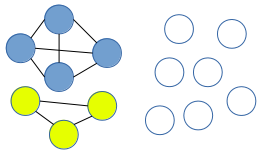
\includegraphics[scale=0.5]{graph}
\caption{Train and test parts of dataset.}
\end{figure}

DCA provided fully anonymized browser logs for a set of devices. A browsing log containing a list of events for a specific device. Each event includes URL (hashed), title (hashed), timestamp.

Example:

\begin{itemize}
\item URL: ed95a9a5be30e4c8/5162fc6a223f248d/

31a42ef13edf7d8a/c2ee3aa455c8b288/
	
656e9a1b3fa15996
\item title: b687bc71fc33713b 19475eb9e8506115

1c202a1bece8798 0e415cc3f3ea206

f27b5d716eb58ac 37a20a398fae482a
\item timestamp: 1464769462076 
\end{itemize}

The hashing is done by replacing all words in the URL and title with their hash-codes. To hash URLs and titles, organizers: 
\begin{enumerate}
\item build the vocabulary by concatenating all available textual data such as URLs and titles;
\item for each unique word, assign a hash-code using an MD5-based hash function;
\item replace each word with the corresponding hash-code.
\end{enumerate}

URL words separated by "/" and "?". Title words separated by spaces.

For example, if we have 2 URLs:
\begin{itemize}
\item google.com/search?text=cats
\item google.com/search?text=dogs
\end{itemize}
First 2 URL words are equal, so their hashes are equal too. For example:
\begin{itemize}
\item 123456/abcdef?10ab10
\item 123456/abcdef?23cd23
\end{itemize}

Also, organizers provided edges for the train part of dataset. Participants should predict edges in the test part.

Here is statistics provided by organizers, so, we know count of correct edges in test part. It's interesting, but not very useful for my solution.

\begin{itemize}
\item The number of unique tokens in titles (dictionary size): 8,485,859
\item The number of unique tokens in URLs (dictionary size): 27,398,114
\item The average number of events/facts per userID: 197
\item The median number of events/facts per userID: 106
\item The number of unique domain names: 282,613
\item The number of all events for all users combined: 66,808,490
\item The number of unique userIDs: 339,405
\item The number of unique websites (domina + URL path): 14,148,535
\item The number of users in the train set: 240,732
\item The number of users in the test set (public and private leaderboard combined): 98,255
\item Known matching pairs for training: 506,136
\item Known matching pairs for testing (public and private leaderboard combined): 215,307
\end{itemize}
 
\begin{figure}
\centering
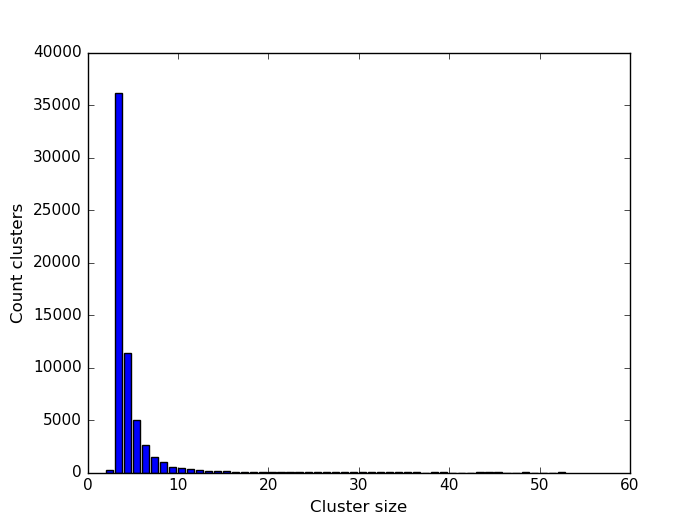
\includegraphics[scale=0.5]{1}
\caption{Count clusters of each size.}
\end{figure}

\subsection{Metric}
Predicted edges were evaluated by $F_1$ score (a harmonic mean of Precision and Recall).
$$F_1=\frac{2pr}{p+r}$$

But there were two phases in contest. 50\% of the correct pairs were used for the first phase and 50\% were used for the second phase during the final stage of the Challenge. So, in each phase half of submitted edges is useless. If we have precision $p$ in validation set, in test set (leaderboard) it will be only $p/2$.
$$F_1^*=\frac{0.5pr}{0.5p+r}$$

It is formula of calculating leaderboard $F_1^*$ score by real precision and recall.

\subsection{Cluster sizes}

We can see on Figure 2, that there very few clusters contain more than 15 devices. But the more devices in cluster, the more edges ($O(N^2)$). And because of metrics calculates $F_1^*$ for edges, we should consider importance of cluster sizes by count of edges in clusters of each size (Figure 3).

\begin{figure}
\centering
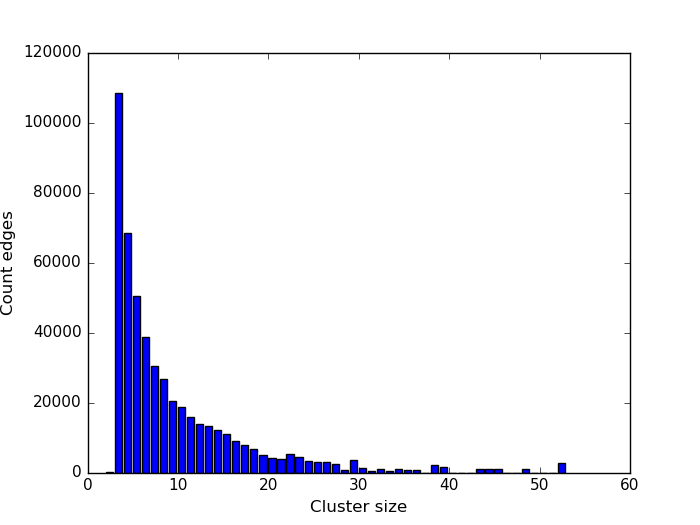
\includegraphics[scale=0.5]{2}
\caption{Count edges in clusters of each size.}
\end{figure}
\begin{table*}
\centering
\caption{Recall and size (in millions)}
\begin{tabular}{|l|l|l|l|l|} \hline
M & K=1 & K=2 & K=3 & K=4\\ \hline
2 & 0.1727 (0.9m) & 0.0878 (0.15m) & 0.0537 (0.07m) & 0.0368 (0.04m)\\ \hline
3 & 0.2405 (1.8m) & 0.1367 (0.32m) & 0.0904 (0.14m) & 0.0647 (0.08m)\\ \hline
5 & 0.3105 (3.5m) & 0.1884 (0.65m) & 0.1291 (0.29m) & 0.0947 (0.17m)\\ \hline
7 & 0.3536 (5m) & 0.2210 (0.9m) & 0.1538 (0.43m) & 0.1138 (0.26m)\\ \hline
10 & 0.3964 (7.3m) & 0.2543 (1.4m) & 0.1795 (0.64m) & 0.1342 (0.38m)\\ \hline
20 & 0.4769 (14m) & 0.3221 (2.9m) & 0.2341 (1.3m) & 0.1785 (0.79m)\\ \hline
30 & 0.5181 (21m) & 0.3587 (4.5m) & 0.2658 (2m) &  0.2053 (1.2m)\\ \hline
50 & 0.5634 (34m) & 0.4035 (7.7m) & 0.3042 (3.4m) & 0.2375 (2m)\\ \hline
70 & 0.5873 (46m) & 0.4260 (10m) & 0.3249 (4.6m) & 0.2561 (2.7m)\\ \hline
100 &  & 0.4520 (14m) & 0.3487 (6.3m) & 0.2769 (3.7m)\\ \hline
150 &  &  & 0.3763 (9m) & \\ \hline
\hline\end{tabular}
\end{table*}

\subsection{Baseline}
Organizers also provided baseline solution. It includes these steps:
\begin{itemize}
\item split urls into words
\item build matrix devices-words
\item process matrix with TF-IDF
\item for each device select 15 nearest neighbours
\item sort all these pairs by distance
\item submit top-215307 best pairs
\end{itemize}
Leaderboard score is \textbf{0.056}.

\bigskip
\section{The approach}
\subsection{Validation dataset} 
Count of submissions was limited by 15/day. So, we decided to create validation dataset to check my ideas without submission. To create it, we retrieved all clusters from train dataset and selected for validation dataset random set of clusters, which has count of edges approximately equal to count of edges in test dataset. Rest clusters included in train dataset.
\subsection{Workflow}
\begin{enumerate}
\item select sample, which contains not many edges (<50 mlns), but with big recall
\item feature extraction
\item learn model and predict probabilities for validation and test dataset
\item divide top-N probabilities into complete subgraphs with MCL (pick N and parameters of MCL in validation dataset)
\end{enumerate}
\subsection{Sample with big recall}
We want to reduce problem to classic machine learning problem i.e. to objects-features matrix, where objects are edges. But there are too many possible edges, for example in train dataset:
$$\frac{339405\cdot339404}{2}\approx5\cdot10^{10}$$
So, we want select subset, which has big recall and is small enough, that we can train model in a reasonable time.

Consider only rare events, which can be found only at $\leqslant M$ devices. Then consider pairs of edges, which have at least K common rare events.

Recall and sizes of such subsets for different K and M are in Table 1.
 
For first iteration we selected samples (K=1, M=30), (K=2, M=50), (K=3, M=50) and all pairs from baseline for 30 nearest neighbours. Union of these sets has recall 0.62 on  train and validation datasets and recall 0.59 on test dataset.
\begin{table*}
\centering
\caption{Results for various pe, pi, p, T on validation set}
\begin{tabular}{|l|l|l|l|} \hline
p, T & pe = 2, pi = 2 & pe = 2, pi = 2.2 & pe = 2, pi = 2.4 \\ \hline
p=0.07, T=30 & 0.42310 & 0.42268 & 0.42116\\ \hline
p=0.10, T=30 & 0.42337 & 0.42298 & 0.42170\\ \hline
p=0.13, T=30 & 0.42323 & 0.42301 & 0.42177\\ \hline
p=0.07, T=40 & 0.42551 & 0.42505 & 0.42416\\ \hline
p=0.10, T=40 & \textbf{0.42587} & 0.42545 & 0.42476\\ \hline
p=0.13, T=40 & 0.42569 & 0.42541 & 0.42478\\ \hline
p=0.07, T=50 & 0.42520 & 0.42523 & 0.42455\\ \hline
p=0.10, T=50 & 0.42552 & 0.42574 & 0.42525\\ \hline
p=0.13, T=50 & 0.42536 & 0.42571 & 0.42525\\ \hline

\hline\end{tabular}
\end{table*}

\subsection{Feature extraction}
For each pair I have created these features:
\begin{itemize}
\item distance in nearest neighbours
\item for 1st vertex order of 2nd among all nearest neighbours (by distance)
\item for 2nd vertex order of 1st among all nearest neighbours (by distance)
\item for each K in Table 1, least M such that pair appear in sample (4 features)
\item URLs: count common with repetition, count commot unique, count common URLs that belong to only 2 devices, count common URLs that belong to only 3 devices, count common URLs that belong to only 4 devices, count common URLs that belong to only 5 devices, count common URLs that belong to only 6-10 devices (7 features)
\item same 7 features for URL words
\item same 7 features for URL domain
\item same 7 features for URL domain + second word
\item same 7 features for titles
\item same 7 features for title words
\item same 7 features for title bigrams
\end{itemize}

It's 56 features total.

\subsection{Model training} 
For training I used Random Forest and selected max tree depth on validation dataset. Best max tree depth is 30.

ROC AUC score on validation dataset is 0.957.

Leaderboard score is \textbf{0.3584}.

\subsection{Sample with big recall - iteration 2} 
Now, we have non-full graph, where each edge has probability. Instead of 4th item in workflow we decided complete connected component of graph and add resulting edges to sample in item 1; then repeat feature extraction and training. First of all, we should limit edges of graph, because it's one big connected component. Algorithm of build limited graph is:
\begin{itemize}
\item sort edges by probability in descending order
\item add each edge to graph in this order except 2 cases
\begin{enumerate}
\item do not add edge, if its probability is less than $p$
\item do not add edge, if it unite components and product of sizes of these components is more than $T$
\end{enumerate}
\end{itemize}

Selecting best $p, T$ on validation dataset, we have best $p=0$(so, it's useless, because all probabilities $\geqslant0$), $T=400$. Recall of these edges is 0.77 on validation dataset. 

For second iteration we selected all these edges from complete subgraphs, samples (K=1, M=70), (K=2, M=100), (K=3, M=150), (K=4, M=100) from Table 1 and all pairs from baseline for 200 nearest neighbours.

Using the same features and model we have leaderboard score \textbf{0.3702}.

\subsection{MCL}
The MCL algorithm based on simulation of random walks within a graph. It is iterative algorithm with 3 main steps: column normalization, expansion, inflation. 

Column normalization is needed to make graph matrix a column stochastic matrix (matrix elements are probabilities, sum in each column is 1).

Expansion is the step, that simulates random walks within a graph, it's only taking the power of a stochastic matrix.

Inflation changes the probabilities after random walks by taking the power of each element. It makes big probabilities bigger and small probabilities smaller.
 
Full algorithm of clustering includes 2 steps:
\begin{itemize}
\item split graph into connected components (like in previous section)
\item apply MCL to each component
\end{itemize}

This algorithm has 4 parameters: $p, T$, power of inflation ($pi$), power of expansion($pe$). Then we select these parameters on validation dataset. In Table 2 are results for some sets of parameters.

Best parameters are $pe=2, pi=2, 0 = 0.10, T=40$.

Leaderboard score is \textbf{0.418}.

Private leaderboard score is \textbf{0.401} (4th place).

\begin{thebibliography}{2}
\bibitem{Contest}
Challenge page. https://competitions.codalab.org/competitions/11171
\bibitem{RF}
Random Forest in sklearn. http://scikit-learn.org/stable/modules/ensemble.html
\bibitem{MCL}
Markov Clustering Algorithm. http://www.micans.org/mcl/
\bibitem{last}
\end{thebibliography}

\end{document}
